\section{Introduction}
\label{introduction}

% state the learning objective 

\section{Introduction}
\label{introduction}

% state the learning objective 
\par The aim of this laboratory assignment is to analyse a RC circuit, which contains a sinusoidal voltage source $v_s$ and a capacitor $C$. The other components present in this four mesh circuit are 7 resistors (from $R_1$ to $R_7$) and a linearly dependent current $I_b$ and voltage $V_d$ sources.
\par The voltage controlled current source depends on the constant $K_d$ and the current controlled voltage source has a linear dependence on the constant $K_b$.

\par The voltage source varies in time as it follows:

\begin{equation}
	v_s(t) = V_s u(-t) + sin(2 \pi f t)u(t)
	\label {equation:n1}
\end{equation}
where
\begin{equation}
	u(t)=e
	\begin{cases}
		0 & $t$ < $0$ \\
		1 & $t $\geq$ 0$
	\end{cases}
	\label {eq:n2}
\end{equation}

\par The data generated automatically by the Python script is given in the table below.

\begin{table}[ht]
  \centering
  \begin{tabular}{|l|r|}
    \hline    
    {\bf Name} & {\bf Value} \\ \hline
    R1 & 1.041113e+03 \\ \hline
R2 & 2.099452e+03 \\ \hline
R3 & 3.131091e+03 \\ \hline
R4 & 4.119470e+03 \\ \hline
R5 & 3.115588e+03 \\ \hline
R6 & 2.047994e+03 \\ \hline
R7 & 1.027544e+03 \\ \hline
Vs & 5.068716e+00 \\ \hline
C & 1.041275e-06 \\ \hline
Kb & 7.287471e-03 \\ \hline
Kd & 8.115684e+03 \\ \hline

  \end{tabular}
  \caption{Initial data generated by Python script. All variables are expressed in Ohms, V, F, S or A.}
  \label{tab:initial_data}
\end{table}



\par The nodes (from $V_1$ to $V_8$) are displayed as it shows in Figure \ref{fig:circ_inicial}. The fourth node is considered to be the ground one.


\par 
   

\par 
In Section 1, for $t < 0$, the voltage and the currents in all branches were determined with the node method. The circuit is analysed by simulations using the program Ngspice. In Section 2, both the equivalent resistor $R_eq$, seen from the capacitor terminals, and the nodes voltage were computed. An operating poin analysis is used to analyse the circuit when $t$ < $0$ and also to determine the time constant.The natural solution is determined in the interval [0, 20]ms in Section 3, followed in the next section with the computation of the forced solution.Both natural and forced solutions are computed with a transiet analysis. These solutions were superimposed. Phasors were converted to real time functions. In Section 6, the voltage ($v_c$, $V_s$ and $V_6$) responses due to variation of frequencies were studied. Theoretical analysis are made in all of the sections. Frequency analysis are also made. All the Ngspices simulations are compared with the theoretical results.
The conclusions of this study are outlined in the final section.



\begin{figure}[ht] \centering
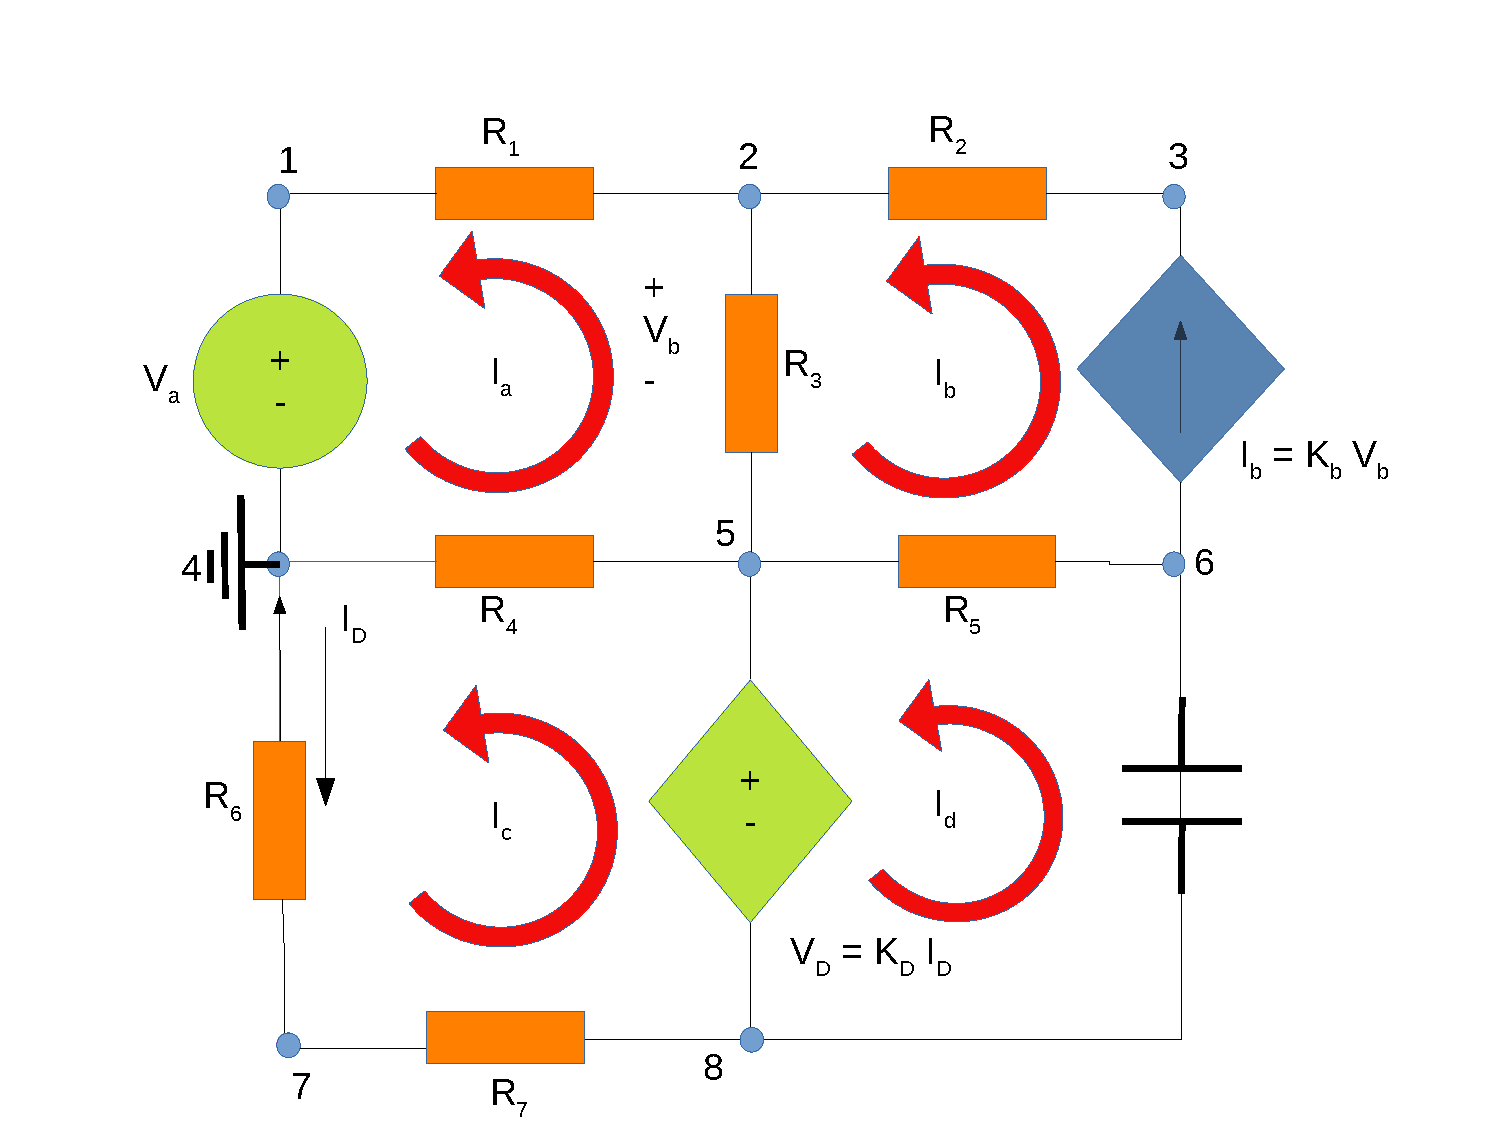
\includegraphics[width=0.9\linewidth]{t2draw.pdf}
\caption{Circuit analysed.}
\label{RC Circuit.}
\end{figure}

















